\section{A new Emulation Technique Based on Bits Relative Sensitivity
for SRAM FPGAs}
\label{intro}
% no \IEEEPARstart

The purpose of this work is to  studying the role of relative sensitivity ratio difference between the configuration bits set to "1" and those set to "0" to produce the highly accurate fault behavior as expected in the real-time radiation testing environment. Because the work  done in~\citep{souari2016towards}, showed that if we considered the bits relative sensitivity difference, i.e., the bits at "1" are more sensitive than the bits at "0", meaning, bits set to "1" are more likely to generate faults than the bits set at "0", we get more realistic results, closer to the radiation-based experiments. 
In this work, the new fault emulation technique is introduced. This technique is based on the bits relative sensitivity, and its features, i.e., bits set to "1" and bits set to "0", in addition, the bits are either LUT or non LUT bits.  We observed that the signature computed by relative sensitivity-based method is $97.8$\% closer to adder circuit signature and $99.4$ \% closer to multiplier circuit signature observed from the radiation based experiment.
This work is the extension of the previous work and make the following contributions. 

\textbf{Contributions:} 
\begin{itemize}

\item{Developed a realistic fault emulation technique in the configuration memory
of FPGAs based system}.
\item{In this work, we propose a fault injection method by using relative sensitivity values between the bits features: e.g., bits belong to LUT at "0", bits belong to LUT at "1", bits belong to Non-LUT at "0", bits belong to Non-LUT at "1"}.
\item{Zero-signature has been derived by flipping the bits-at-1, bits-at-0, randomly, flipped the bits based on the relative sensitivity between bits-at-1, bits-at-0, and relative sensitivity between bits-status and their features}.
\end{itemize}


\section{Methodology}
\label{Methodology}
The emulation of SEUs in an FPGA is done by flipping the bit in the configuration memory by using the IP provided by the Xilinx named - SEM core~\citep{xilinx}. The emulation platform used in this work was designed for the radiation experiment~\citep{hobeika2014multi}. In this work, this platform is employed for the fault emulation. The platform comprises of two Artix-7 FPGAs. The "Reference-Board" comprises of the original design, e.g., 16-bit adder and 8-bit multiplier. The design under "Test-Board" is subjected to fault emulation.  

\subsection{Identification of the Sensitivity bits}
\label{SE-bits}
The first step is the identification of the bits (the bit address and the bit location). The identification of the bits is important in our work because we want to emulate such a fault injection experiment that produce the same result as expected in the real experiment.
I developed some tools that extract the bit address and the bit location from the \textit{.rbd }file of the design. The \textit{.rbd} an ASCII file that contains readback data, including pad words and frames.
The proposed procedure is shown in Figure~\ref{fig:original-rbd}, and Figure~\ref{fig:inverted-rbd}.  I used two tools for this purpose: 
\begin{itemize}
\item Xilinx ISE tool to generate the \textit{.ncd} file and \textit{.xdl} file of the design that helps to find the bits feature which bits belongs to LUT and which are non-LUT bits.
\item I used Vivado tool to get the \textit{.rbd} file of the design from the FPGA.


\end{itemize}

The classification of the bits consists of following steps:
\begin{itemize}
\item Generate the \textit{.ncd} file of the design, generate the original \textit{.bit} file, downloaded the \textit{.bit} file into the FPGA and used the vivado \textit{readback} command to read the original \textit{.rbd} file as shown in Figure~\ref{fig:original-rbd}.
\item Then from the \textit{.ncd} file of the design generate the \textit{.xdl} file of the design  which contains placement information of primitive sites, and their routing regarding switch matrix connections.
\item Python script has been developed that inverts all the logic of LUTs in the \textit{.xdl} file, and generates the modified \textit{.ncd} file, and modified \textit{.bit} file as shown in Figure~\ref{fig:inverted-rbd}.
\item Once we get both two files, we further investigated to find the bits features that which bits belong to the LUTs and which are non-LUTs bits.
\item Algorithm~\ref{BCA} describe the feature extraction procedure. For example, if the bit is at state "one" in the original \textit{.rbd} file and it's being detected "zero" in the inverted \textit{.rbd} file means bit belongs to the LUT bits at "one" represented as (L1)." Similarly, for non-lut-at-0 (NL0), non-lut-at-1 (NL1), and lut-at-0 (L0). 
\end{itemize}

\begin{figure}[tb!]
 \centering
  \captionsetup{justification=centering}    
   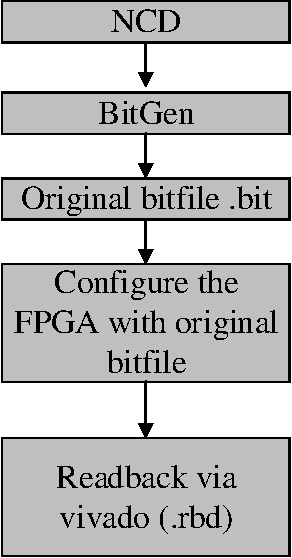
\includegraphics[scale = 0.5]{Figures/original-rbd.pdf}
   \caption{Procedure to extract the original .rbd file}
\label{fig:original-rbd}
\end{figure}
\begin{figure}[tb!]
 \centering
  \captionsetup{justification=centering}    
   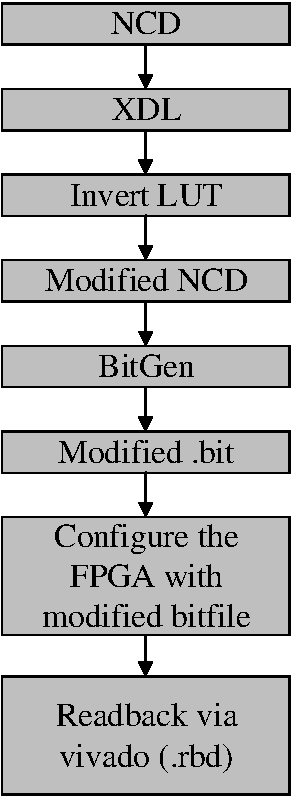
\includegraphics[scale = 0.5]{Figures/inverted-rbd.pdf}
   \caption{Procedure to extract the inverted LUT .rbd file}
\label{fig:inverted-rbd}
\end{figure}


\begin{algorithm}
\caption{Bits classification algorithm.}
\begin{algorithmic}
\label{BCA}
\REQUIRE $.rbd$ $original$ $and$ $.rbd$ $inverted$ \\
%\textbf{Compute}\\ 
%\hspace{1.5cm}{$Original =  A $ $ \times $ $ B$ } \\
%\hspace{1.5cm}{$Faulty =  A $ $ \times $ $ B$ } \\
%\vspace{0.20 cm }
%\textbf{Stuck-at-1:}
\vspace{0.20 cm }
\IF{$Original$  $ = $ $ 0 $  $Inverted$ $==$ $0$}
\vspace{0.10 cm }
\STATE \textit{ NL0 = Not LUT bits at 0}
\vspace{0.10 cm }
\ELSIF{$Original$  $ = $ $ 0 $  $Inverted$ $==$ $1$}
\vspace{0.10 cm }
\STATE \textit{ L0 = LUT bits at 0}
\vspace{0.10 cm }
\ELSIF{$Original$  $ = $ $ 1 $  $Inverted$ $==$ $0$}
\vspace{0.10 cm }
\STATE \textit{ L1 =  LUT bits at 1}
\vspace{0.10 cm }
\ELSIF{$Original$  $ = $ $ 1 $  $Inverted$ $==$ $1$}
\vspace{0.10 cm }
\STATE \textit{ NL1 = Not LUT bits at 1}
\vspace{0.10 cm }


\ENDIF
\vspace{0.20 cm }
\end{algorithmic}
\end{algorithm}



\section{Experimental Results}
\label{Experimental Results}
In this section, we will discuss the result of emulation performed by flipping the bits at "1" and at "0." We experimented with fifty different runs. Each run provides $6,144$ signatures further subdivided into three different groups. 
Table~\ref{AE}, and Table~\ref{ME} show the percentage of the zero signatures, e.g., $00000000$ for adder and multiplier. The maximum number of zero signatures observed for flip-at-0. The number of bits flipped observed; $65,750$ among them $150$ bits are critical bits with the statistical ratio of $0.22\%$ critical bits at $0$. The minimum number of zero signatures observed for bits flip-at-1, with the total flipped bits are $1,356$ among $3,110,418$ non-BRAM bits. In this case, the critical bits at $1$ are $11.06\%$. 
Similarly, for the multiplier,  the number of bits flipped observed are $29,752$ with total non-BRAM(bits-at-0) are $56,771,430$ giving the statistical ratio of $0.50\%$ critical bits at $0$. The minimum number of zero signatures observed for bits flip-at-1, with the total flipped bits are $1,664$ among $3,750,970$ non-BRAM bits. In this case, the critical bits at $1$ are $9.01\%$.

Then the emulation performed with the random fault injection, in which we randomly combined the bits-at-1, and the bits-at-0 and calculated the zero signatures. As expected, the random injection zero-signature value should lower than the flip-at-0 and higher than the flip-at-1 because the number of bits at "0" are $18.45$ times higher than the bits at "1" for adder and  $15.13$ for multiplier. The purpose of performing the random injection is to compare the result with the relative sensitivity results and experimentally prove that by considering the relative sensitivity of the bits more realistic results are produced. The bit flip ratio observed in the random injection (flip-at-0 to flip-at-1) is $18.10$ for the adder as shown in Table~\ref{RI} and $15.15$ for the multiplier as shown in Table~\ref{RIM}. This bit-flip information indicates that the bit flip in random mode is valid. Next, we performed the relative sensitivity experiment named SA-01, and SA-02.
In SA-01, we used the relative sensitivity concept that the  bits-at-1 are $2.11$ times more sensitive than the bit-at-0~\citep{souari2016towards}. In this emulation, we get the $7.95\%$ difference with the irradiation experiment for the adder \footnote{need some more tests} and $1.58\%$ for the multiplier. The total bit flips we observed for adder are: $9,807$ among them $8,797$ flipped-at-0 and $1,010$ for flipped-at-1. Similarly, for the multiplier, the total bits flipped are $7,227$ among them $6,345$ flipped-at-0 and $882$ flipped-at-1. Both emulations give us a bit flipped ratio of $2.11$ proved that emulation setup is valid. 





\begin{table}[tb!]
\center
\caption{Adder Emulation Tests Comparison.}
\label{AE}
\begin{tabular}{|c | c| c | c| c| c |} 
 \hline
Test & Zero Signature (\%) & Difference with Radiation (\%)   \\ 
\hline
 
 
 Flip@1& 49.0 &22.5   \\
 \hline
 Flip@0 & 62.8 & 2.2 \\ 
 \hline
 
 Random & 58.1 & 5.5  \\
 \hline
 SA-01 & 56.7 & 7.95\\
 \hline
 SA-02 & 60.1 & 2.13 \\
 \hline
 Radiation & 61.4 & 0  \\
 \hline
 
 
\end{tabular}
\end{table}

\begin{table}[tb!]
\center
\caption{Multiplier Emulation Tests Comparison.}
\label{ME}
\begin{tabular}{|c | c| c | c| c| c |} 
 \hline
Test & Zero Signature (\%) & Difference with Radiation (\%)   \\ 
\hline
 
 
 Flip@1& 62.0 &18.3   \\
 \hline
 Flip@0 & 76.0 & 1.9 \\ 
 \hline
 
 Random & 72.1 & 3.3  \\
 \hline
 SA-01 & 73.4 & 1.5 \\
 \hline
 SA-02 & 74.9 &  0.5\\
 \hline
 Radiation & 74.6 & 0  \\
 \hline
 
 
\end{tabular}
\end{table}



\begin{table}[tb!]
\center
\caption{Adder Random Injection Bits Information.}
\label{RI}
\begin{tabular}{c c  c c   } 
 \hline
\multicolumn{2}{c}{Bit}     & Flip Ratio (Theoretical) &  Flip Ratio (Observed)   \\ 
%\hline
%& \multicolumn{1}{c}{ (Theoretical)} \\
%& & \multicolumn{1}{c}{observed} \\
 \hline
 
 Bits@0 & $57 411 982  $ & \multirow{2}{*}{18.45} & \multirow{2}{*}{18.10} \\
 %\hline
 Bits@1 & $3110418$  & &\\ 
 \hline
% 
% Bits@0 LUT & 2.06 &2.08 &2.096\\
% \hline
% Bits@1 LUT & 1.91 &1.92&1.91\\
 %\hline
% \hline
 
 
\end{tabular}
\end{table}

\begin{table}[tb!]
\center
\caption{Multiplier Random Injection Bits Information.}
\label{RIM}
\begin{tabular}{c c  c c   } 
 \hline
\multicolumn{2}{c}{Bit}     & Flip Ratio (Theoretical) &  Flip Ratio (Observed)   \\ 
%\hline
%& \multicolumn{1}{c}{ (Theoretical)} \\
%& & \multicolumn{1}{c}{observed} \\
 \hline
 
 Bits@0 & $57 411 982  $ & \multirow{2}{*}{15.93} & \multirow{2}{*}{15.15} \\
 %\hline
 Bits@1 & $3110418$  & &\\ 
 \hline
% 
% Bits@0 LUT & 2.06 &2.08 &2.096\\
% \hline
% Bits@1 LUT & 1.91 &1.92&1.91\\
 %\hline
% \hline
 
 
\end{tabular}
\end{table}


Then, we further investigated the bits feature, i.e., bits belong to LUT and non-LUT bits. We used the bits relative sensitivity values shown in Table~\ref{RS}. The result we obtained by using this approach indicates only $2.13\%$ difference for adder and $0.50\%$ for multiplier suggests that by considering bits sensitivity with bits features more realistic results can be achieved, and better fault emulation can be performed. 

%\begin{table}[tb!]
%\center
%\caption{Adder Emulation Tests Comparison.}
%
%\label{AE}
%
%\begin{tabular}{|c | c| c | c| c| c |} 
% \hline
%Test & Zero Signature (\%) & Difference with Radiation (\%)   \\ 
%\hline
%
% 
% 
% Flip@1& 49.048 &22.53   \\
% \hline
% Flip@0 & 62.801 & 2.095 \\ 
% \hline
% 
% Random & 59.378 & 3.51  \\
% \hline
% SA-01 & 60.36 & 1.87 \\
% \hline
% SA-02 & 60.559 &1.47  \\
% \hline
% Radiation & 61.499 & 0  \\
% \hline
% 
% 
%\end{tabular}
%\end{table}


We also measured the relative sensitivity (experimentally validated) and the bit flip information for this emulation setup shown in the Table~\ref{RS} to prove the bit flip emulation validity. Table~\ref{RSflipA} and~\ref{RSflipM} shows the bit flip information for the adder and multiplier respectively.

\begin{table}[tb!]
\center
\caption{Relative Sensitivity from experimentation performed at TRIUMF.}
\label{RS}
\begin{tabular}{|c | c| c | c | } 
 \hline
Bits feature & \makecell*{Relative Sensitivity}  & \makecell*{Adder \\(Observed)} & \makecell*{Multiplier \\ (Observed)}  \\ 
%\hline
%& \multicolumn{1}{c}{ (Theoretical)} \\
%& & \multicolumn{1}{c}{observed} \\
 \hline
 
 Bits@0 non LUT & 1.00 & 1.00 & 1.00 \\
 \hline
 Bits@1 non LUT& 1.41  & 1.43&1.44\\ 
 \hline
 
 Bits@0 LUT & 2.06 &2.08 &2.09\\
 \hline
 Bits@1 LUT & 1.91 &1.92&1.91\\
 \hline
% \hline
 
 
\end{tabular}
\end{table}









\begin{table}[tb!]
\center
\caption{Bit Flip Ratio Relative Sensitivity (Adder).}
\label{RSflipA}
\begin{tabular}{|c | c| c | c | } 
 \hline
Bits feature & \makecell*{Bit Flip)}  & \makecell*{Bit Flip Ratio\\(Total)} \\ 
%\hline
%& \multicolumn{1}{c}{ (Theoretical)} \\
%& & \multicolumn{1}{c}{observed} \\
 \hline
 
 Bits@0 non LUT & 5251  & 1.00  \\
 \hline
 Bits@1 non LUT& 236  & 1.43\\ 
 \hline
 
 Bits@0 LUT & 266 &2.08 \\
 \hline
 Bits@1 LUT & 245 &1.92\\
 \hline
% \hline
 
 
\end{tabular}
\end{table}

\begin{table}[tb!]
\center
\caption{Bit Flip Ratio Relative Sensitivity (Mull).}
\label{RSflipM}
\begin{tabular}{|c | c| c | c | } 
 \hline
Bits feature & \makecell*{Bit Flip}  & \makecell*{Bit Flip Ratio\\(Total)} \\ 
%\hline
%& \multicolumn{1}{c}{ (Theoretical)} \\
%& & \multicolumn{1}{c}{observed} \\
 \hline
 
 Bits@0 non LUT & 8833  & 1.00  \\
 \hline
 Bits@1 non LUT& 454  & 454\\ 
 \hline
 
 Bits@0 LUT & 603 &2.09\\
 \hline
 Bits@1 LUT & 553 &1.91\\
 \hline
% \hline
 
 
\end{tabular}
\end{table}


\section{Conclusions}

In this work, sensitivity of the configuration bits has been considered along with the bits feature to
produced results as close as possible to those obtained by the accelerated tests. 

\label{Conclusion}